\begin{figure}[ht]
    \centering
    \vspace{2em}
    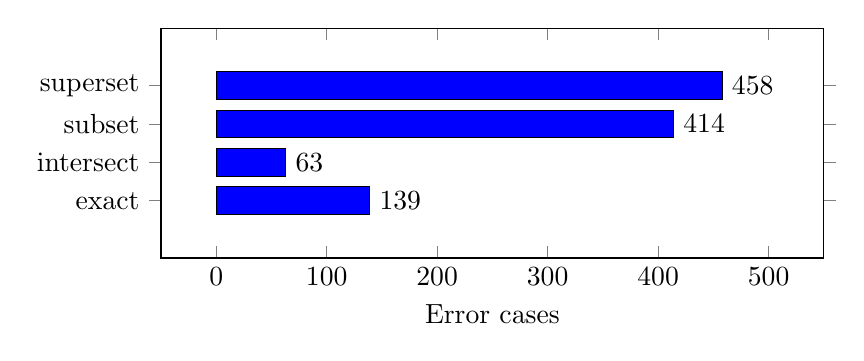
\begin{tikzpicture}
        \begin{axis}[
            enlarge y limits=0.5,
            enlarge x limits=0.1,
            height=4.5cm,
            width=10cm,
            symbolic y coords={
            exact,intersect,subset,superset
            },
            xmin=0,
            xmax=500,
            xbar=1pt,
            xlabel=Error cases,
            nodes near coords={\pgfmathprintnumber[/pgf/number format/assume math mode]{\pgfplotspointmeta}},
            nodes near coords align={horizontal},
            every node near coord/.append style={
                anchor=west}
            ,
            xticklabel style={/pgf/number format/assume math mode},
            yticklabel style={/pgf/number format/assume math mode},
            ytick=data
          ]
            \addplot[xbar,fill=blue] coordinates {
            (458,superset)
            (414,subset)
            (63,intersect)
            (139,exact)
            };
        \end{axis}
    \end{tikzpicture}
    \caption{\label{i:argument-error-type} Error cases for argument extraction
        by the relationship with the real interval. }
\end{figure}
